\documentclass[a4paper,12pt]{article}
\usepackage{geometry}
\usepackage[english]{babel}
\usepackage[utf8]{inputenc}
\usepackage{amsmath}
\usepackage{sectsty}
\usepackage{indentfirst}
\usepackage{placeins}
\sectionfont{\centering}
%\usepackage{graphicx}
%\usepackage[nottoc,notlot,notlof]{tocbibind}
\usepackage{tocbasic}
\usepackage[colorinlistoftodos]{todonotes}

\geometry{a4paper,total={170mm,257mm},left=26mm,top=25mm,bottom=20mm}
\renewcommand{\baselinestretch}{1.0}
\graphicspath{ {images/} }

\title{\textbf{Exploring Fatal Police Shootings\\
\large{Data Visualization}
}}

\author{Felix Kikaya}

\date{\today}

\begin{document}

\maketitle

\begin{abstract}
While crime seems to have declined in some areas in the last few years, the number of police related shootings seem to have been on the rise. High profile cases such the shooting of Michael Brown\cite{ferguson} in Ferguson, Missouri and Laquan McDonald in Chicago, Illinois, have not only drawn so much controversy, but also brought great attention to matters of policing within our society. These cases have poignantly filled majority of newspapers, television stations, as well as a variety of social media platforms and the discussions are endless. With this, movement groups such as Black Lives matter have prompted inquiries about "use of force" and whether there is bias on how police make "shoot or don't shoot" decisions. Using data, a large number of police departments and agencies have found the impetus to analyze and study the effect of race on the officers decisions - while looking at other relevant factors. Studies have shown that there exists a disproportionate number of fatal shootings within minority groups compared to whites, something majority of the communities hasn't been able to has struggle to discern. This project attempts to look at a sample of documented fatal shootings from 2015 to 2018 while paying attention to race and other relevant factors. 
\end{abstract}
%\newpage
%\tableofcontents

%\newpage
\section{Introduction}
Police brutality has been a contentious subject that is rooted into the history of the United States for many decades. It is not often that such a subject would occur without touching into matters of racial bias and the effect it has on police judgment. Recent advancements in technology such as proliferation of hand-held mobile devices have enabled an almost real-time sharing of information and shown quite a number of cases regarding how policing was being carried out in society. Another advancement has been the use of body cameras which police officers have been required to wear while on duty especially when interacting with a suspect. While such technologies where not utilized in the past, data on such interactions were virtually non-existent. Most cases were either not well documented or not reported at all. 
 
In this era of information science, it is important to utilize the resources that are readily available in our societies to study such cases. Using data, a more knowledgeable approach can be given to the issue. Researchers at different agencies such as the Guardian, the vice, and the Washington Post have spearheaded the initiative to collect data from fatal and non-fatal shootings from different police departments across the country. These agencies, however, are still faced with challenges, such as data not being public or some departments not providing all the events that lead to shooting of the suspect. This project will focus on data specifically collected by the Washington Post\cite{fatal_force}.

\section{Background}
The Post \cite{washington_post},began tracking details of each police shootings starting January of 2015, including the circumstances that led up to the shooting. The focused on attributes such as race, age, sex, state, city, armed or unarmed e.t.c. They also searched for documentation on whether the officer was equipped with a body camera prior to the shooting or not. The Washington Post's databases get updated regularly as they receive information on shootings as they get reported.

To add onto the Washington Post's fatal shooting data-set, data pulled from four other databases will be used. These will help analyze other relevant factors such as racial composition and population, poverty levels in the community - including median income and level of education, Including other factors that often determine the magnitude of crime in communities. It is expected that when poverty level are high while education is low, crime would be high. This can also have an influence into the police officers judgment of the events leading to the shooting\cite{deadly_force}. 

However, much information on the police officer is not provided besides use of body camera. It is important to note that some basic information on the officer can better help see there is indeed a trend. Factors such as race, age, sex, and experience of the officer are some of the things not reported are some of the things not reported.

\section{Objectives}
The main objective of this project will be to determine that, if adjusted to population, what is the proportion of different race groups involved in fatal police shootings. This will be determined by the population of the individual race groups in relation to the number of fatal shootings. Other objects are listed as follows;
\begin{itemize}
  \item Determine and compare the number of fatal shootings among different cities. The top ten cities with the highest number of fatal shootings will also be computed. With this, the racial composition of the population will be studied.
  \item The use of body camera in on year to year basis will be analyzed to determine if there has been an increase or a decrease in usage as a result of the recent campaigns.
  \item A distribution of the age of the suspects will be explored while also looking at the gender.
  \item A visualization of median income levels across all the states will be plotted to determine poverty levels as a factor that contributes to crime levels. Change in poverty levels versus percentage of people that have completed high school will be evaluated to determine if there is a direct relationship between education and poverty.
  \item Since mental state of the suspects has been a component in such discussions, cases of mental illness will be determined in each racial group. This will determine how many suspects were mentally ill and also whether they were armed, and what kind of weapon they had.
\end{itemize}
Other objectives will be drawn as the data is being explored.
\section{Data Visualization Tools}
Data visualization will be conducted using Python programming language. The python visualization landscape is quite large. It comes with many libraries that can be used to create beautiful plots for visualization and analyses. Most plots are shared are usually shared between multiple libraries. The architecture of the each library can be determined by attributes such as the size of the data\cite{python}. The huge range is mostly based on functionality and diversity in approach. In this project we will focus on using Matplotlib, Seaborn, Plotly, and Folium visualization libraries. 

Matplotlib is one of the oldest library, released in 2003. It is equipped with quite and extensive range or 2D formats and plotting types. It is also the most popular of the other libraries. Seaborn is built on Matplotlib and comes with great themes that can be used for styling informative plots. It helps simplify complicated plots. Plotly is an interactive tool for visualization that is used for scientific plotting. It is easy to interact with and extract and visualize the data. Folium\cite{folium} on the other hand is built on the strength of the python programming language and is great for binding data to maps and chloropleth visualizations. Jupyter notebooks an open source web application for interactive computing was also used for integrating all these technologies together.

\section{Process Analysis}
Exploratory data analysis methods as well as statistical analysis method were all put together to bring insight from the five datasets. The datasets were downloaded from their respective sources and imported into the Jupyter notebooks environment as a dataframe using pandas. Basic information about the datasets was then extracted to derive information such as column data types, size of the columns, presence of null and missing values.

To prepare the data for analysis, certain parts of the data had to be cleaned out to prepare it for processing. Non-categorical value columns had to be converted from object to float for computation. The column headers were changed to the same format and unnecessary characters removed from them. Data cleaning also involved removing unnecessary text from categorical columns. 

\section{Results and Discussion}
This section looks at plots and visualizations that were derived from the data using python libraries. It is important to note that the results only represent information based on the collected data. They are not a conclusion of given events. 
\subsection{Median Income Across States}
This plot is a chlorepleth map showing the income variation across different states in the US. Folium library was used to create this. It was preferred over plotly since the latter took longer to load the map and would at times make jupyter notebooks freeze. Folium on the other hand was faster and easier to implement. It also provided an option of viewing the plot in an html format over the browser. According to Figure 1. below, the states with the highest median income are New Jersey, New York, Indiana, Oaklahoma, and California.

\begin{figure}[hbt!]
    \centering
    \includegraphics[width=1.0\textwidth]{map.png}
    \caption{}
\end{figure}
\FloatBarrier

\subsection{Effect of Education on Median Income}
Higher education levels typically tend to reflect higher levels of income. However, they don't usually consider completion high school and other training that influence things like salary and rates of unemployment. The higher the unemployment rate, the higher the poverty levels and therefore chances of getting involved in crime. The plot below shows a trend in the direction at which median income takes with a change in high school completion. The median incomes seems to tend lower as the completion rate goes lower and vice-versa. Texas had the lowest high school completion rate while Mississippi had the lowest median income. On the other hand, New Jersey had the highest median income while Massachusetts had the highest high school completion rate. This observation can be evidenced with the fact that majority of people that work in New York City tend to live in New Jersey and that Boston has one of the the biggest school districts in the U.S.

\begin{figure}[hbt!]
    \centering
    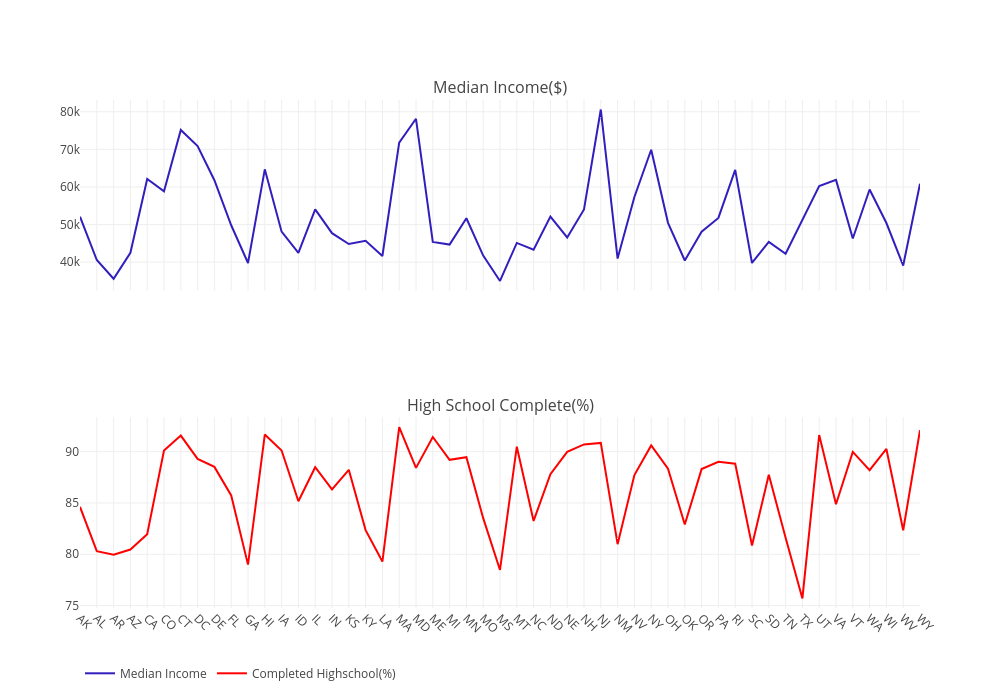
\includegraphics[width=0.8\textwidth]{income-subplots-shared-yaxes.png}
    \caption{}
\end{figure}
\FloatBarrier

\subsection{Effect of Education on Poverty Levels}
\begin{figure}[hbt!]
    \centering
    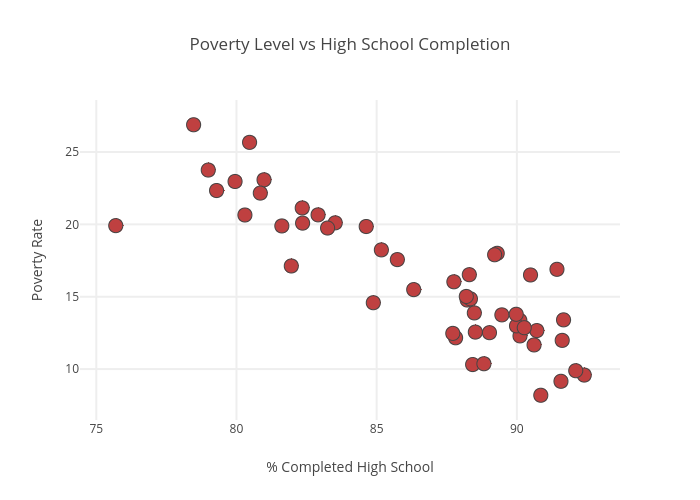
\includegraphics[width=0.8\textwidth]{poverty_vs_high_school.png}
    \caption{}
\end{figure}
\FloatBarrier
It has been seen that poverty also shows a direct relationship with high school completion. Figure 3. above is a distribution of change in poverty rate against high school. The scattered data points seem to possess a linear relationship with a negative gradient. The plot in Figure 4 below includes a fitted regression line that shows the direction of change with an increase in high school completion. Poverty rate decreases with increase in number of people that complete high school. Typically employees with less that high school degrees are the lowest earners. The inability to secure a professional position as well as lack of adequate qualifications play a role in ability to be employed and how much pay can be taken home. 
\begin{figure}[hbt!]
    \centering
    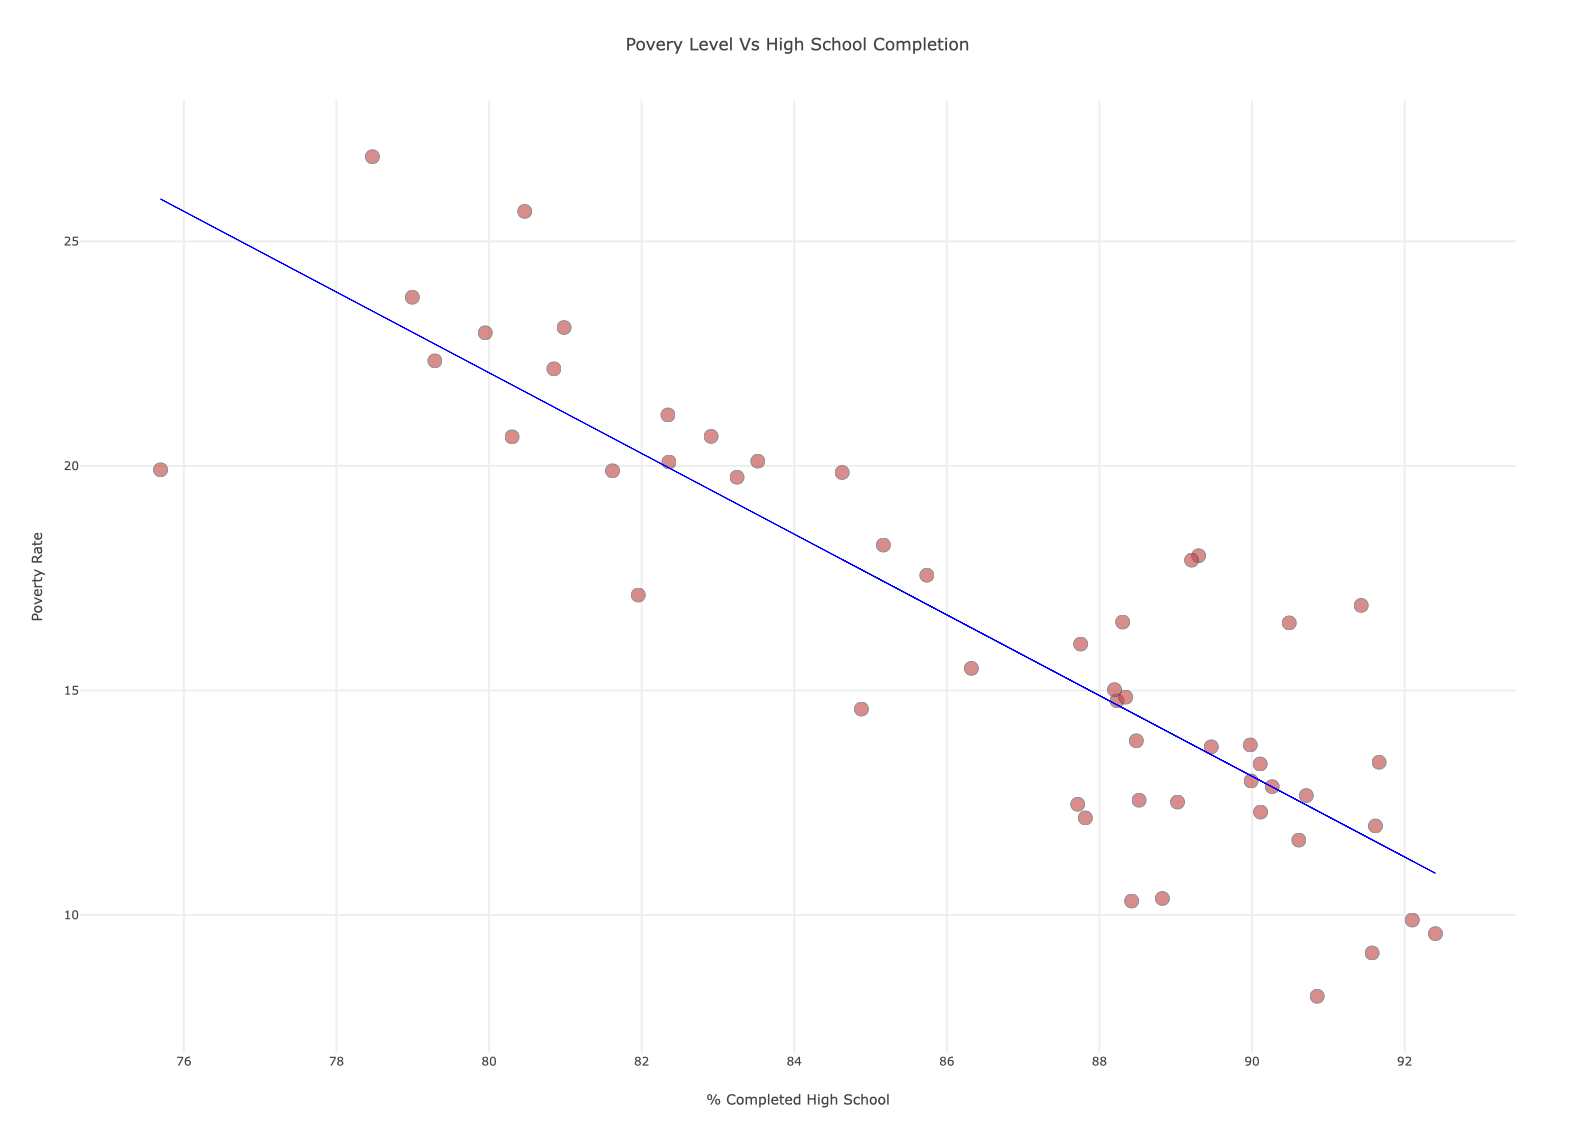
\includegraphics[width=0.8\textwidth]{plot_from_API.png}
    \caption{}
\end{figure}
\FloatBarrier

\subsection{Fatal Shooting Distributions}
The subplots below provide a sneak peak into the fatal shootings dataset from the Washington Post. The number of people tasered then shot was significantly lower than those whom were shot at the instant. About 3,500 were shot and 250 shot and tasered and a majority of them were between 20 and 60 years old. White, Black, and Hispanic formed majority of the population by a significant difference. Many of the deceased suspects were armed with guns or a knife. Not many of them were unarmed. It can therefore be seen that most of the suspects posed some kind of a threat. 

It is possible that both the suspect and the police officer could provide contradicting of false details of what occurred. It is also true that in the case of a fatal shooting, the dead cannot tell their story. One is left with only one story and that is the story of the shooter. Video footage provides investigators objective details of incidents\cite{camera}. Though they cannot provide the full details of the event, they can significantly tell what exactly happened during the incident. Hence the reason why dash-board and body camera have been proposed by many organizations and continue to be a campaign when it comes to this subject. So has the use of body cameras been increasing over the years? Figure 6. below shows there hasn't been a significant change. There were slightly more body cameras used in 2016 but the rest the years show not much of a difference. Infact, there is almost no difference between 2017 and 2018.
\begin{figure}[hbt!]
    \centering
    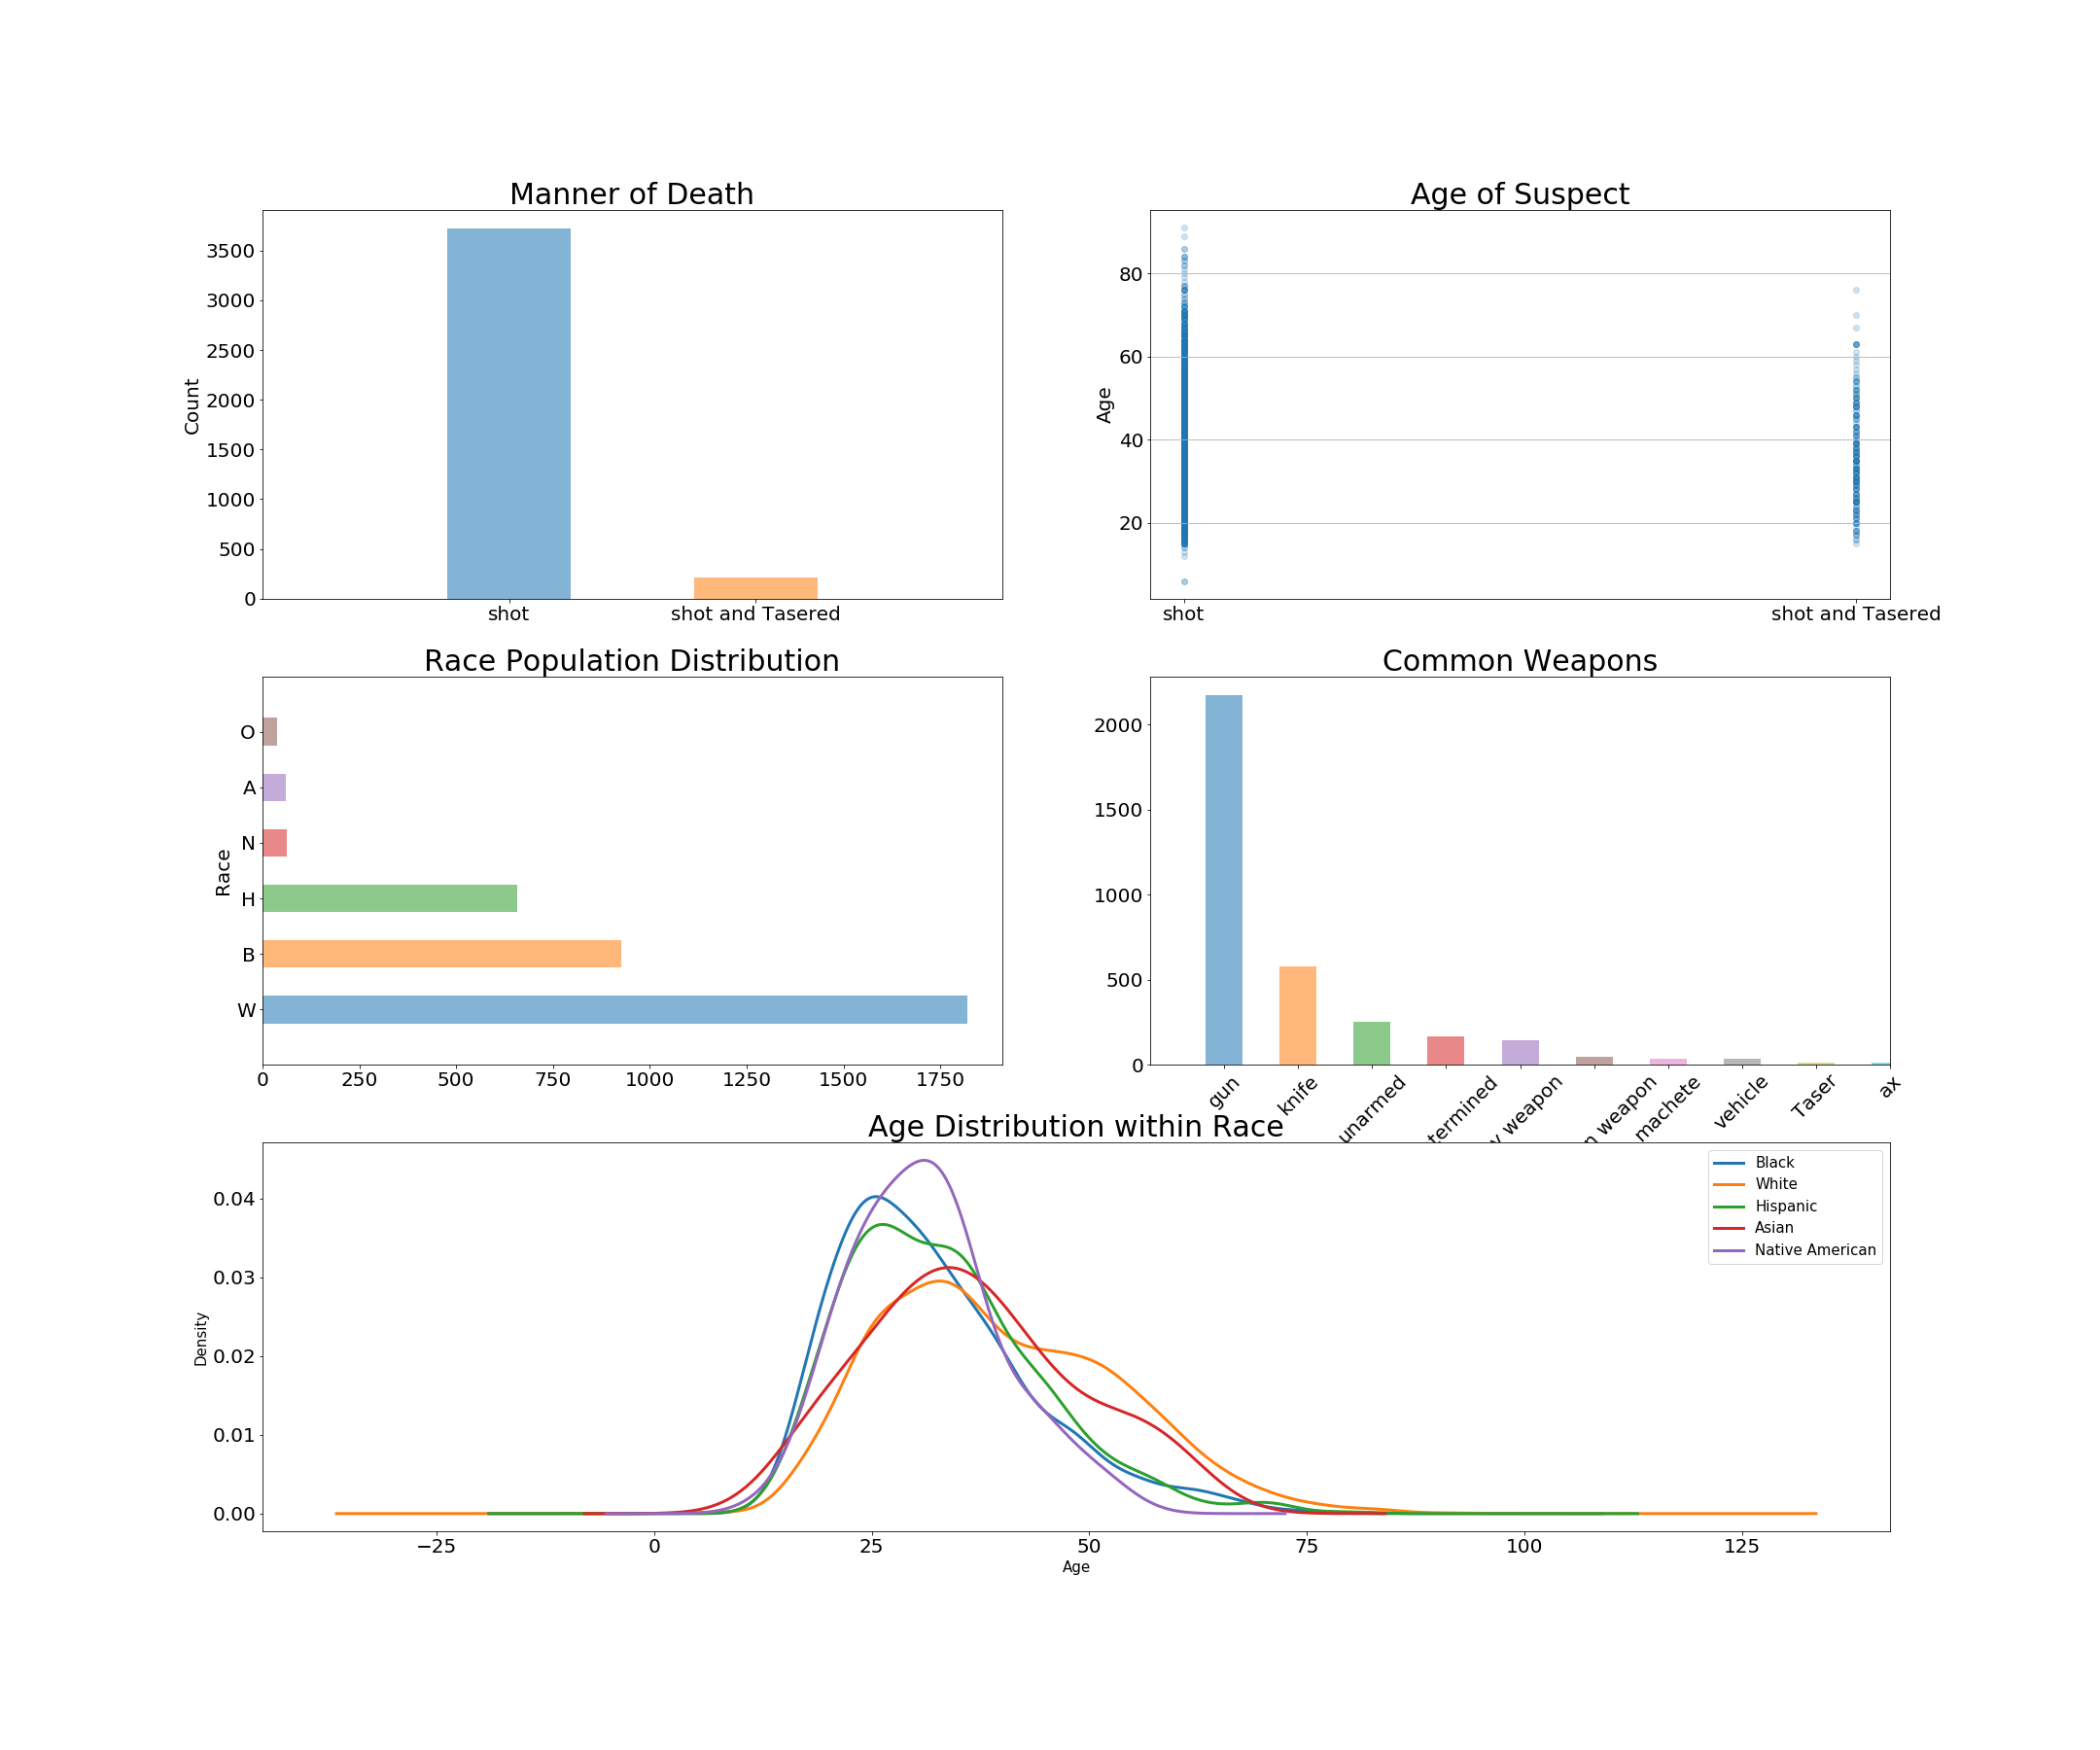
\includegraphics[width=1.0\textwidth]{distribution_plots.png}
    \caption{}
\end{figure}
\FloatBarrier

\begin{figure}[hbt!]
    \centering
    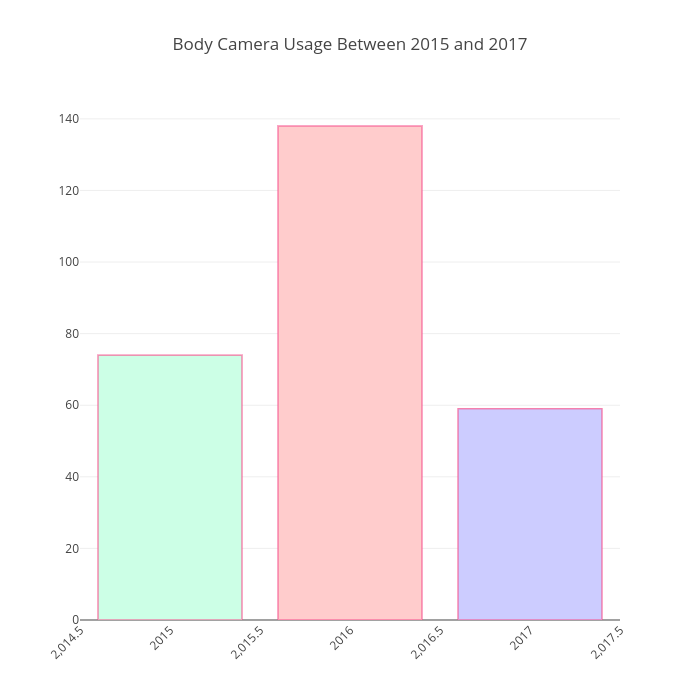
\includegraphics[width=0.5\textwidth]{body_camera.png}
    \caption{}
\end{figure}
\FloatBarrier

\subsection{Cases of Mental Illness in Racial Groups}
\begin{figure}[hbt!]
    \centering
    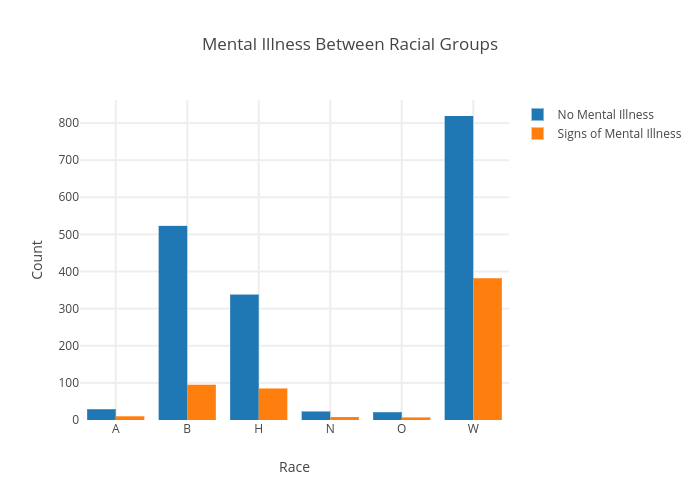
\includegraphics[width=1.0\textwidth]{mental_image_plot.png}
    \caption{}
\end{figure}
\FloatBarrier

\subsection{Racial Populations}
\begin{figure}[hbt!]
    \centering
    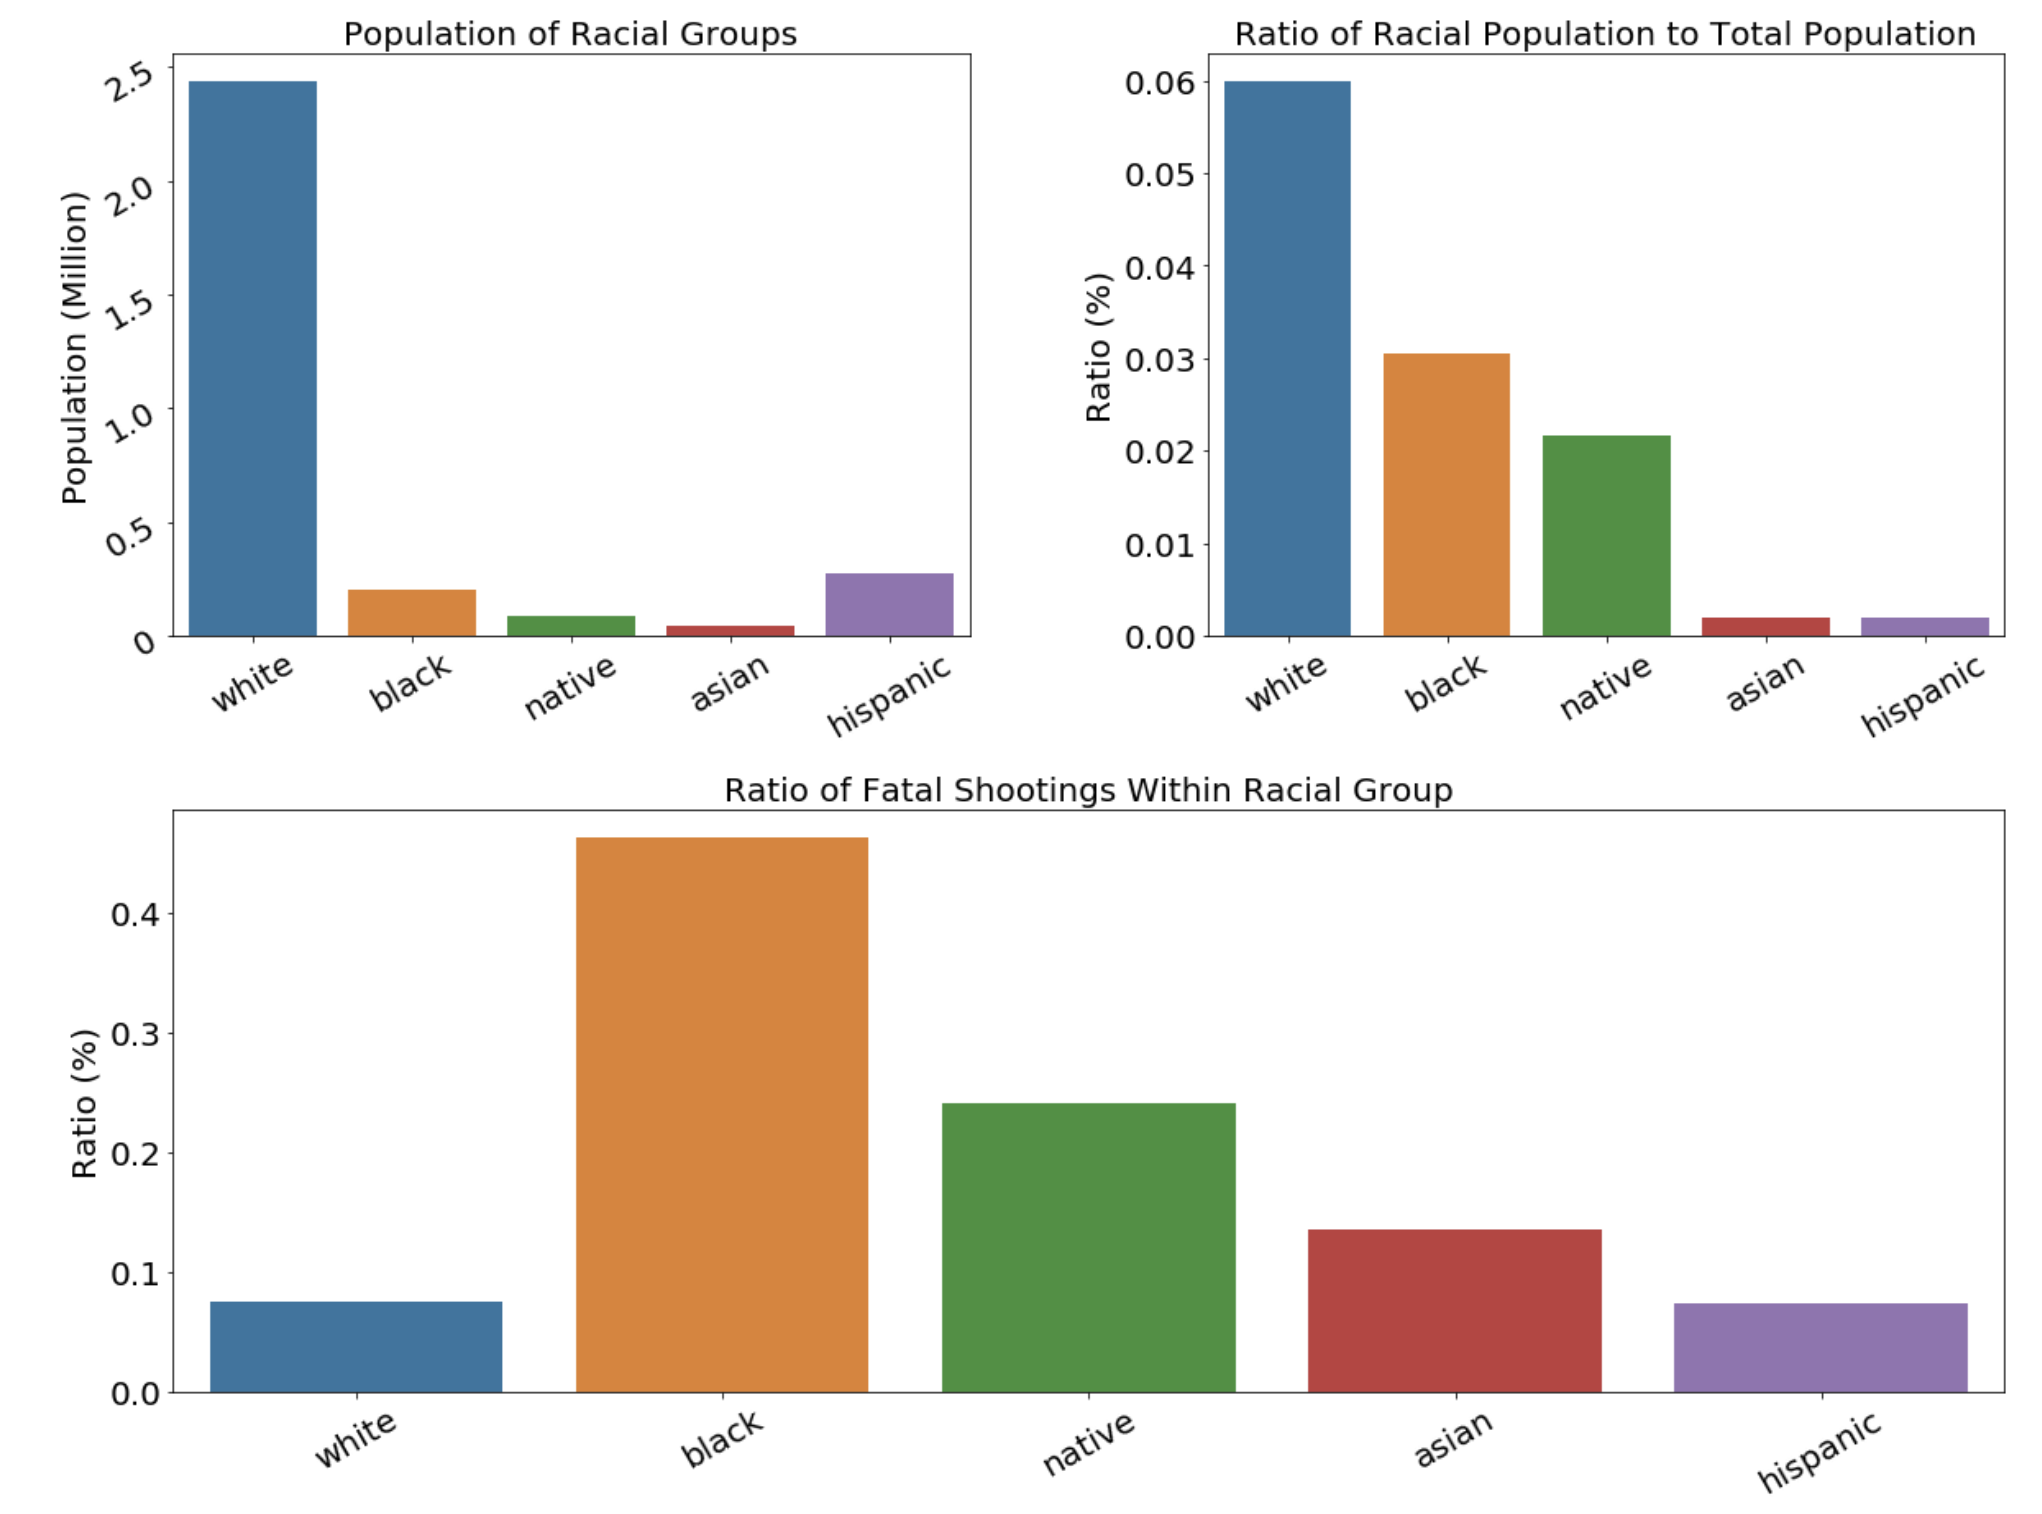
\includegraphics[width=1.0\textwidth]{populaton_ratios.png}
    \caption{}
\end{figure}
\FloatBarrier

\subsection{Fatalities Based on Gender}
\begin{figure}[hbt!]
    \centering
    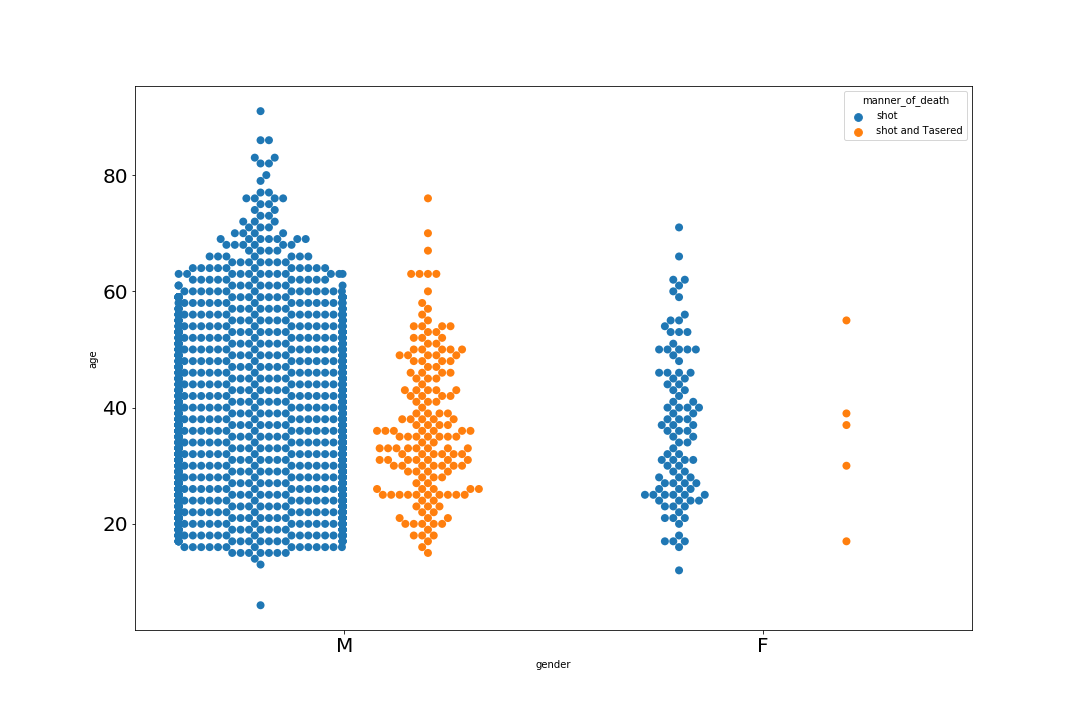
\includegraphics[width=1.0\textwidth]{swarm_plot_death.png}
    \caption{}
\end{figure}
\FloatBarrier
\subsection{Cities with Highest Fatalities}

\begin{figure}[hbt!]
    \centering
    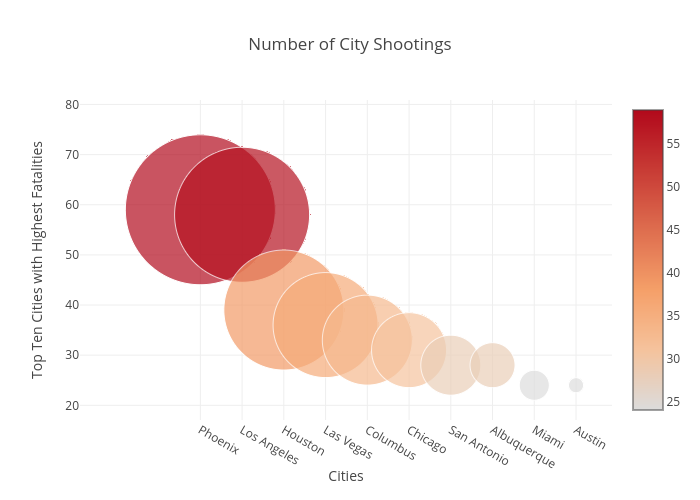
\includegraphics[width=1.0\textwidth]{Number_of_city_shootings.png}
    \caption{}
\end{figure}
\FloatBarrier

\section{Conclusion}
There is a disproportionate number of shootings in the minority group
\section{Future work}
A lot of work is yet to be done in collecting the data

\bibliographystyle{plain}
\bibliography{fatal}

\end{document}